% Source: Code/yolo-ablation-bench/report.tex
% Description: At 320px, all models achieve 23--26 FPS. YOLOv8l slightly faster due to better GPU utilization.

\documentclass[border=4pt]{standalone}
\usepackage[T1]{fontenc}
\usepackage{graphicx}
\usepackage{helvet}
\usepackage{lmodern}
\usepackage{pgfplots}
\usepackage{pgfplotstable}
\usepackage{tikz}
\usepackage[dvipsnames,table]{xcolor}
\pgfplotsset{compat=1.18}

\definecolor{garnet}{HTML}{73000A}
\definecolor{midgray}{gray}{0.35}
\definecolor{lightgray}{gray}{0.8}


\newcommand{\headline}[1]{\textcolor{garnet}{\Large\bfseries #1}}
\newcommand{\subhead}[1]{\textcolor{midgray}{\large #1}}
\newcommand{\bulletline}[1]{\noindent\textcolor{midgray}{\textbullet}\ #1\\[-0.2em]}

\begin{document}
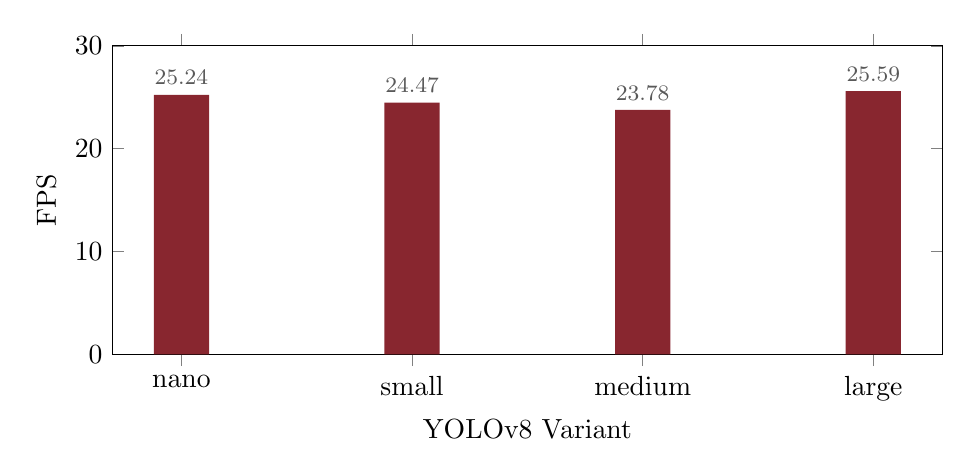
\begin{tikzpicture}
    \begin{axis}[
      width=\textwidth,
      height=5.5cm,
      ybar,
      bar width=20pt,
      xlabel={YOLOv8 Variant},
      ylabel={FPS},
      symbolic x coords={nano,small,medium,large},
      xtick=data,
      nodes near coords,
      every node near coord/.style={font=\footnotesize, color=midgray, anchor=south},
      ymin=0, ymax=30
    ]
      \addplot+[fill=garnet!85, draw=none] coordinates {
        (nano, 25.24) (small, 24.47) (medium, 23.78) (large, 25.59)
      };
    \end{axis}
  \end{tikzpicture}
\end{document}
